\input{../../../../.preambles/02-lab_work}
\input{../../../../.preambles/20-math}
\newgeometry{top=1.5cm, bottom=1.5cm, left=1cm, right=1cm}
\begin{document}
    \begin{table}[h!]
        \center
        \begin{tabular}{|C{.5}|C{.2}|C{.25}|}
            \hline
            \multicolumn{1}{|c|}{\multirow{4}{*}{Лабораторная работа № 3}} &
            Студент, группа & \\ \cline{2-3}
            & Дата выполнения & 23.09.2013 \\ \cline{2-3}
            & Подпись &  \\ \cline{2-3}
            Исследование статических & Дата отчёта & \\ \cline{2-3}
            характеристик триода & Оценка &  \\ \cline{2-3}
            & Подпись &  \\ \hline
        \end{tabular}
    \end{table}

    \emph{Цель работы:} изучение методов определения статических характеристик
    триода и изучение режимов его работы.
    
    \begin{figure}[h!]
        \center
        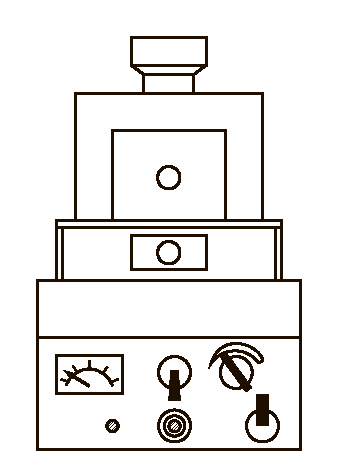
\includegraphics[width=.45\textwidth]{appearance} \hspace*{2em}
        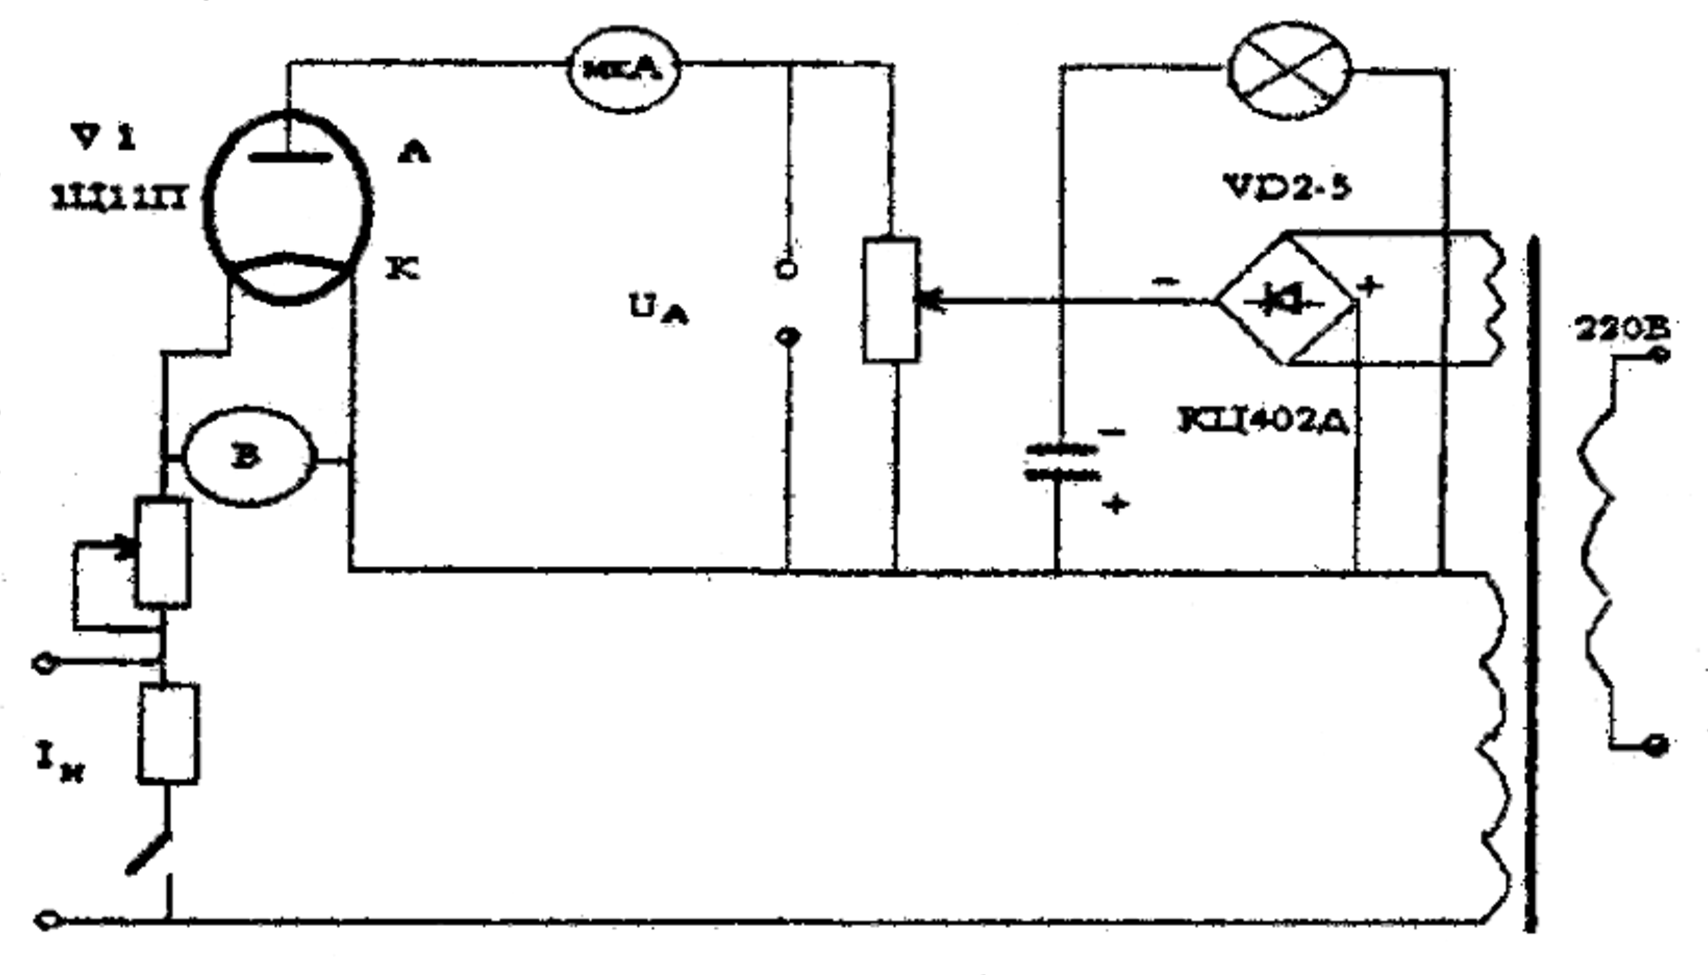
\includegraphics[width=.4\textwidth]{scheme}
        \parbox{.45\textwidth}{\caption{Внешний вид экспериментального макета}}
        \hspace*{2em}
        \parbox{.4\textwidth}{\caption{Принципиальная электрическая схема
        экспериментальной установки}}
    \end{figure}
    
    \begin{table}[h!]
        \center
        \caption{Семейство анодно-сеточных характеристик}
        \begin{tabular}{|m{.1\textwidth}|*{8}{C{.07}|}} \hline
        \multirow{5}{*}{\( U_{a_{01}} =  90 \)~В} & \( U_c \),~В &
            -1,2 & -1,0 & -0,8 & -0,6 & -0,4 & -0,2 & 0 \\ \cline{2-9}
        & \( I_{a_1} \),~мА &
            0 & 0,4 & 0,8 & 2,0 & 4,4 & 7,6 & 13,2 \\ \cline{2-9}
        & \( I_{a_2} \),~мА &
            0 & 0,4 & 0,8 & 2,4 & 4,8 & 8,0 & 13,2 \\ \cline{2-9}
        & \( I_{a_3} \),~мА &
            0 & 0,4 & 0,8 & 2,4 & 4,4 & 9,2 & 13,2 \\ \cline{2-9}
        & \( \midnum{I_a} \),~мА &
            0 & 0,4 & 0,8 & 2,3 & 4,5 & 8,3 & 13,2 \\ \hline
        \multirow{5}{*}{\( U_{a_{02}} = 100 \)~В} & \( U_c \),~В &
            -1,4 & -1,2 & -1,0 & -0,8 & -0,6 & -0,4 & -0,2 \\ \cline{2-9}
        & \( I_{a_1} \),~мА &
            0 & 0,4 & 0,8 & 1,6 & 3,2 & 6,4 & 12,0 \\ \cline{2-9}
        & \( I_{a_2} \),~мА &
            0 & 0,4 & 0,8 & 1,6 & 3,6 & 6,0 & 12,0 \\ \cline{2-9}
        & \( I_{a_3} \),~мА &
            0 & 0,4 & 0,8 & 1,6 & 3,2 & 6,0 & 12,0 \\ \cline{2-9}
        & \( \midnum{I_a} \),~мА &
            0 & 0,4 & 0,8 & 1,6 & 3,3 & 6,1 & 12,0 \\ \hline
        \multirow{5}{*}{\( U_{a_{03}} = 120 \)~В} & \( U_c \),~В &
            -2,0 & -1,4 & -1,0 & -0,8 & -0,6 & -0,4 & -0,2 \\ \cline{2-9}
        & \( I_{a_1} \),~мА &
            0 & 0,4 & 1,6 & 3,6 & 6,4 & 10,8 & 16,8 \\ \cline{2-9}
        & \( I_{a_2} \),~мА &
            0 & 0,4 & 1,6 & 3,6 & 6,4 & 11,2 & 16,4 \\ \cline{2-9}
        & \( I_{a_3} \),~мА &
            0 & 0,4 & 1,6 & 3,6 & 6,4 & 10,8 & 16,4 \\ \cline{2-9}
        & \( \midnum{I_a} \),~мА &
            0 & 0,4 & 1,6 & 3,6 & 6,4 & 10,9 & 16,5 \\ \hline
        \multirow{5}{*}{\( U_{a_{04}} = 140 \)~В} & \( U_c \),~В &
            -2,0 & -1,6 & -1,2 & -1,0 & -0,8 & -0,6 & -0,4 \\ \cline{2-9}
        & \( I_{a_1} \),~мА &
            0 & 0,4 & 2,0 & 4,0 & 6,4 & 10,8 & 16,4 \\ \cline{2-9}
        & \( I_{a_2} \),~мА &
            0 & 0,4 & 2,0 & 4,0 & 7,2 & 11,6 & 16,8 \\ \cline{2-9}
        & \( I_{a_3} \),~мА &
            0 & 0,4 & 2,0 & 3,6 & 6,8 & 11,2 & 16,0 \\ \cline{2-9}
        & \( \midnum{I_a} \),~мА &
            0 & 0,4 & 2,0 & 3,9 & 6,8 & 11,2 & 16,4 \\ \hline
        \end{tabular}
    \end{table}
    
    \pagebreak
    
    \begin{table}[h!]
        \center
        \caption{Семейство анодных характеристик триода}
        \begin{tabular}{|m{.12\textwidth}|C{.07}|*{9}{C{.05}|}} \hline
        \multirow{5}{*}{\( U_{c_{01}} = -2,0 \)~В} & \( U_a \),~В &
            140 & 180 & 190 & 200 & 210 & 220 & 230 & 240 & 250 \\ \cline{2-11}
        & \( I_{a_1} \),~мА &
            0 & 0,4 & 1,2 & 1,6 & 2,0 & 3,2 & 4,0 & 5,2 & 6,8 \\ \cline{2-11}
        & \( I_{a_2} \),~мА &
            0 & 0,4 & 1,2 & 1,6 & 2,0 & 3,2 & 4,0 & 5,2 & 6,8 \\ \cline{2-11}
        & \( I_{a_3} \),~мА &
            0 & 0,4 & 0,8 & 1,6 & 2,0 & 2,8 & 4,0 & 5,2 & 6,4 \\ \cline{2-11}
        & \( \midnum{I_a} \),~мА &
            0 & 0,4 & 1,1 & 1,6 & 2,0 & 3,1 & 4,0 & 5,2 & 6,7 \\ \hline
        \multirow{5}{*}{\( U_{c_{02}} = -1,5 \)~В} & \( U_a \),~В &
            120 & 130 & 150 & 160 & 175 & 185 & 195 & 220 & 250 \\ \cline{2-11}
        & \( I_{a_1} \),~мА &
            0 & 0,4 & 1,2 & 1,6 & 2,8 & 4,0 & 5,6 & 10,0 & 16,8 \\ \cline{2-11}
        & \( I_{a_2} \),~мА &
            0 & 0,4 & 1,2 & 2,0 & 3,2 & 4,0 & 5,6 & 10,0 & 16,8 \\ \cline{2-11}
        & \( I_{a_3} \),~мА &
            0 & 0,4 & 1,2 & 1,6 & 2,8 & 3,6 & 5,6 & 10,0 & 16,8 \\ \cline{2-11}
        & \( \midnum{I_a} \),~мА &
            0 & 0,4 & 1,2 & 1,7 & 2,9 & 3,9 & 5,6 & 10,0 & 16,8 \\ \hline
        \multirow{5}{*}{\( U_{c_{03}} = -1,0 \)~В} & \( U_a \),~В &
            60 & 95 & 115 & 125 & 140 & 155 & 165 & 185 & 200 \\ \cline{2-11}
        & \( I_{a_1} \),~мА &
            0 & 0,4 & 1,2 & 2,0 & 4,0 & 6,0 & 8,0 & 12,0 & 16,0 \\ \cline{2-11}
        & \( I_{a_2} \),~мА &
            0 & 0,4 & 1,6 & 2,4 & 4,0 & 6,4 & 8,0 & 12,4 & 16,4 \\ \cline{2-11}
        & \( I_{a_3} \),~мА &
            0 & 0,4 & 1,2 & 2,0 & 4,0 & 6,0 & 8,0 & 12,0 & 16,0 \\ \cline{2-11}
        & \( \midnum{I_a} \),~мА &
            0 & 0,4 & 1,3 & 2,1 & 4,0 & 6,1 & 8,0 & 12,1 & 16,1 \\ \hline
        \multirow{5}{*}{\( U_{c_{04}} = -0,5 \)~В} & \( U_a \),~В &
            40 & 55 & 80 & 90 & 105 & 120 & 135 & 140 & 150 \\ \cline{2-11}
        & \( I_{a_1} \),~мА &
            0 & 0,4 & 2,0 & 3,2 & 5,2 & 8,4 & 12,0 & 14,0 & 16,0 \\ \cline{2-11}
        & \( I_{a_2} \),~мА &
            0 & 0,4 & 2,0 & 3,2 & 5,6 & 8,8 & 12,0 & 13,6 & 16,4 \\ \cline{2-11}
        & \( I_{a_3} \),~мА &
            0 & 0,4 & 1,6 & 2,8 & 4,8 & 8,0 & 11,6 & 12,8 & 15,2 \\ \cline{2-11}
        & \( \midnum{I_a} \),~мА &
            0 & 0,4 & 1,9 & 3,1 & 5,2 & 8,4 & 11,9 & 13,5 & 15,9 \\ \hline
        \multirow{5}{*}{\( U_{c_{05}} = 0 \)~В} & \( U_a \),~В &
            0 & 20 & 35 & 45 & 50 & 60 & 70 & 80 & 90 \\ \cline{2-11}
        & \( I_{a_1} \),~мА &
            0 & 0,4 & 1,6 & 2,8 & 4,0 & 6,0 & 8,0 & 10,0 & 14,0 \\ \cline{2-11}
        & \( I_{a_2} \),~мА &
            0 & 0,4 & 1,6 & 2,8 & 3,6 & 5,6 & 8,0 & 10,4 & 13,2 \\ \cline{2-11}
        & \( I_{a_3} \),~мА &
            0 & 0,4 & 1,6 & 2,8 & 3,6 & 5,6 & 8,0 & 10,4 & 13,2 \\ \cline{2-11}
        & \( \midnum{I_a} \),~мА &
            0 & 0,4 & 1,6 & 2,8 & 3,7 & 5,7 & 8,0 & 10,3 & 13,5 \\ \hline
        \end{tabular}
    \end{table}
\end{document}
